\pdfbookmark{Общая характеристика работы}{characteristic}             % Закладка pdf
\section*{Общая характеристика работы}

\newcommand{\actuality}{\pdfbookmark[1]{Актуальность}{actuality}\underline{\textbf{\actualityTXT}}}
\newcommand{\progress}{\pdfbookmark[1]{Разработанность темы}{progress}\underline{\textbf{\progressTXT}}}
\newcommand{\aim}{\pdfbookmark[1]{Цели}{aim}\underline{{\textbf\aimTXT}}}
\newcommand{\tasks}{\pdfbookmark[1]{Задачи}{tasks}\underline{\textbf{\tasksTXT}}}
\newcommand{\aimtasks}{\pdfbookmark[1]{Цели и задачи}{aimtasks}\aimtasksTXT}
\newcommand{\novelty}{\pdfbookmark[1]{Научная новизна}{novelty}\underline{\textbf{\noveltyTXT}}}
\newcommand{\influence}{\pdfbookmark[1]{Практическая значимость}{influence}\underline{\textbf{\influenceTXT}}}
\newcommand{\methods}{\pdfbookmark[1]{Методология и методы исследования}{methods}\underline{\textbf{\methodsTXT}}}
\newcommand{\defpositions}{\pdfbookmark[1]{Положения, выносимые на защиту}{defpositions}\underline{\textbf{\defpositionsTXT}}}
\newcommand{\reliability}{\pdfbookmark[1]{Достоверность}{reliability}\underline{\textbf{\reliabilityTXT}}}
\newcommand{\probation}{\pdfbookmark[1]{Апробация}{probation}\underline{\textbf{\probationTXT}}}
\newcommand{\contribution}{\pdfbookmark[1]{Личный вклад}{contribution}\underline{\textbf{\contributionTXT}}}
\newcommand{\publications}{\pdfbookmark[1]{Публикации}{publications}\underline{\textbf{\publicationsTXT}}}


{\actuality} 
\ifsynopsis
В настоящее время процессы самоорганизации привлекают внимание исследователей из различных областей естествознания: физики, биологии, химии, медицины, экономики (см., например, \cite{field1985oscillations}, \cite{kuramoto1984chemical}). Системы дифференциальных уравнений с диффузией активно используются при математическом моделировании этих процессов \cite{hoyle2006pattern}, \cite{cross2009pattern}. Следуя основополагающей работе Тьюринга \cite{turing1990chemical}, явления самоорганизации с образованием неоднородных паттернов в таких системах обычно связывают с диффузионной неустойчивостью. Трудности идентификации и классификации различных паттернов обусловлены высокой чувствительностью процессов самоорганизации к вариациям параметров и высокой степенью мультистабильности (см., например, \cite{kolinichenko2020multistability}, \cite{bib4} и ссылки в них). Мультистабильность в таких системах приводит к тому, что при одном и том же наборе параметров решения системы стабилизируются к паттернам-аттракторам различной волновой структуры. В этих условиях разработка методов количественного анализа такой неопределенности является сложной задачей для исследователей. В настоящей работе рассматривается проблема анализа неопределенности в сложных диффузионных системах и квантификации особенностей формируемых паттернов и переходных процессов.
\else
Этот абзац появляется только в~диссертации.
Через проверку условия \verb!\!\verb!ifsynopsis!, задаваемого в~основном файле
документа (\verb!dissertation.tex! для диссертации), можно сделать новую
команду, обеспечивающую появление цитаты в~диссертации, но~не~в~автореферате.
\fi

% {\progress}
% Этот раздел должен быть отдельным структурным элементом по
% ГОСТ, но он, как правило, включается в описание актуальности
% темы. Нужен он отдельным структурынм элемементом или нет ---
% смотрите другие диссертации вашего совета, скорее всего не нужен.

{\aim} данной работы является создание и описание методов и подходов, позволяющих эффективно анализировать процессы пространственной самоорганизации в динамических системах с диффузией.

Для~достижения поставленной цели необходимо было решить следующие {\tasks}:
\begin{enumerate}[beginpenalty=10000] % https://tex.stackexchange.com/a/476052/104425
  \item Разработать метод для квантификации переходных процессов и паттернов в случае диффузии на одномерном пространстве.
  \item Апробировать полученный теоретический аппарат на реальных моделях.
  \item Построить обобщение выработаных ранее подходов и методов на случай диффузии на двумерном пространстве.
\end{enumerate}


{\novelty}
\begin{enumerate}[beginpenalty=10000] % https://tex.stackexchange.com/a/476052/104425
  \item Впервые описан подход к квантификации самоорганизации в динамических системах с диффузией на основе множественных численных экспериментов и статистик, построенных на основе гармонических коэффициентов.
  \item Было выполнено оригинальное исследование разнообразия формируемых пространственно неоднородных паттернов в гликолитических осцилляторах Хиггинса, Селькова и Селькова-Строгаца. 
  \item Описан способ автоматической классификации некоторых типов устойчивых двумерных пространственных паттернов, возникающих в динамических системах в присутствии диффузии.
\end{enumerate}

{\influence} состоит в применении разработанных методов к различным моделям гликолиза и выявлении конкретных феноменов самоорганизации в таких моделях. Практическую ценность также представляют разработанные комплексы программ. Теоретическая значимость диссертационной работы заключается в разработанных общих методах анализа переходных процессов и типов формируемых устойчивых паттернов в динамических системах с диффузией и предложенной методике анализа множественных численных экспериментов применительно к таким задачам. 

{\defpositions}
\begin{enumerate}[beginpenalty=10000] % https://tex.stackexchange.com/a/476052/104425
  \item Разработаны новые методы анализа переходных процессов и самоорганизации в динамических системах с диффузией.
  \item Проведено комплексное исследование феноменов самоорганизаци в моделях гликолитического осциллятора Хиггинса, гликолитического осциллятора Селькова и гликолитического осциллятора Селькова-Строгаца.
  \item Предложен и применён для гликолитического осциллятора Хиггинса подход к детекции типа двумерных Тьюринговских паттернов.
\end{enumerate}

{\probation}
Основные результаты работы докладывались в формате устных и стендовых докладов на 12 международных конференциях
\begin{enumerate}
    \item V Международная молодежная научная конференция «Физика. Технологии. Инновации». ФТИ-2018 (14-18 мая 2018 года, г. Екатеринбург)
    \item VI Международная молодежная научная конференция «Физика. Технологии. Инновации». ФТИ-2019 (20-24 мая 2019 года, г. Екатеринбург)
    \item Международная (51-я Всероссийская) молодежная школа-конференция «Современные проблемы математики и ее приложений» (3 — 7 февраля 2020 года, г. Екатеринбург)
    \item VII Международная молодежная научная конференция «Физика. Технологии. Инновации». ФТИ-2020 (18-22 мая 2020 года, г. Екатеринбург)
    \item Международная (52-я Всероссийская) молодежная школа-конференция «Современные проблемы математики и ее приложений» (8 — 12 февраля 2021 года, г. Екатеринбург)
    \item VIII Международная молодежная научная конференция «Физика. Технологии. Инновации». ФТИ-2021 (17-21 мая 2021 года, г. Екатеринбург)
    \item Международная (53-я Всероссийская) молодежная школа-конференция «Современные проблемы математики и ее приложений» (31 января — 4 февраля 2022 года, г. Екатеринбург)
    \item IX Международная молодежная научная конференция «Физика. Технологии. Инновации». ФТИ-2022 (16-20 мая 2022 года, г. Екатеринбург)
    \item XXIX Международная конференция «Математика. Компьютер. Образование» (24 — 28 января 2022 года. Онлайн-конференция)
    \item Международная (54-я Всероссийская) молодежная школа-конференция «Современные проблемы математики и ее приложений» (6 — 10 и 17 февраля 2023 года, г. Екатеринбург)
    \item X Международная молодежная научная конференция «Физика. Технологии. Инновации». ФТИ-2023 (15-19 мая 2023 года, г. Екатеринбург)
    \item Международная (55-я Всероссийская) молодежная школа-конференция «Современные проблемы математики и ее приложений» (29 января — 2 февраля и 16 февраля 2024 года, г. Екатеринбург)
\end{enumerate} 

% {\contribution} Автор принимал активное участие \ldots

\ifnumequal{\value{bibliosel}}{0}
{%%% Встроенная реализация с загрузкой файла через движок bibtex8. (При желании, внутри можно использовать обычные ссылки, наподобие `\cite{vakbib1,vakbib2}`).
    {\publications} Основные результаты по теме диссертации изложены
    в~XX~печатных изданиях,
    X из которых изданы в журналах, рекомендованных ВАК,
    X "--- в тезисах докладов.
}%
{%%% Реализация пакетом biblatex через движок biber
    \begin{refsection}[bl-author, bl-registered]
        % Это refsection=1.
        % Процитированные здесь работы:
        %  * подсчитываются, для автоматического составления фразы "Основные результаты ..."
        %  * попадают в авторскую библиографию, при usefootcite==0 и стиле `\insertbiblioauthor` или `\insertbiblioauthorgrouped`
        %  * нумеруются там в зависимости от порядка команд `\printbibliography` в этом разделе.
        %  * при использовании `\insertbiblioauthorgrouped`, порядок команд `\printbibliography` в нём должен быть тем же (см. biblio/biblatex.tex)
        %
        % Невидимый библиографический список для подсчёта количества публикаций:
        \printbibliography[heading=nobibheading, section=1, env=countauthorvak,          keyword=biblioauthorvak]%
        \printbibliography[heading=nobibheading, section=1, env=countauthorwos,          keyword=biblioauthorwos]%
        \printbibliography[heading=nobibheading, section=1, env=countauthorscopus,       keyword=biblioauthorscopus]%
        \printbibliography[heading=nobibheading, section=1, env=countauthorconf,         keyword=biblioauthorconf]%
        \printbibliography[heading=nobibheading, section=1, env=countauthorother,        keyword=biblioauthorother]%
        \printbibliography[heading=nobibheading, section=1, env=countregistered,         keyword=biblioregistered]%
        \printbibliography[heading=nobibheading, section=1, env=countauthorpatent,       keyword=biblioauthorpatent]%
        \printbibliography[heading=nobibheading, section=1, env=countauthorprogram,      keyword=biblioauthorprogram]%
        \printbibliography[heading=nobibheading, section=1, env=countauthor,             keyword=biblioauthor]%
        \printbibliography[heading=nobibheading, section=1, env=countauthorvakscopuswos, filter=vakscopuswos]%
        \printbibliography[heading=nobibheading, section=1, env=countauthorscopuswos,    filter=scopuswos]%
        %
        \nocite{*}%
        %
        {\publications} Основные результаты по теме диссертации изложены в~\arabic{citeauthor}~печатных изданиях,
        \arabic{citeauthorvak} из которых изданы в журналах, рекомендованных ВАК\sloppy%
        \ifnum \value{citeauthorscopuswos}>0%
            , \arabic{citeauthorscopuswos} "--- в~периодических научных журналах, индексируемых Web of~Science и Scopus\sloppy%
        \fi%
        \ifnum \value{citeauthorconf}>0%
            , \arabic{citeauthorconf} "--- в~тезисах докладов.
        \else%
            .
        \fi%
        \ifnum \value{citeregistered}=1%
            \ifnum \value{citeauthorpatent}=1%
                Зарегистрирован \arabic{citeauthorpatent} патент.
            \fi%
            \ifnum \value{citeauthorprogram}=1%
                Зарегистрирована \arabic{citeauthorprogram} программа для ЭВМ.
            \fi%
        \fi%
        \ifnum \value{citeregistered}>1%
            Зарегистрированы\ %
            \ifnum \value{citeauthorpatent}>0%
            \formbytotal{citeauthorpatent}{патент}{}{а}{}\sloppy%
            \ifnum \value{citeauthorprogram}=0 . \else \ и~\fi%
            \fi%
            \ifnum \value{citeauthorprogram}>0%
            \formbytotal{citeauthorprogram}{программ}{а}{ы}{} для ЭВМ.
            \fi%
        \fi%
        % К публикациям, в которых излагаются основные научные результаты диссертации на соискание учёной
        % степени, в рецензируемых изданиях приравниваются патенты на изобретения, патенты (свидетельства) на
        % полезную модель, патенты на промышленный образец, патенты на селекционные достижения, свидетельства
        % на программу для электронных вычислительных машин, базу данных, топологию интегральных микросхем,
        % зарегистрированные в установленном порядке.(в ред. Постановления Правительства РФ от 21.04.2016 N 335)
    \end{refsection}%
    \begin{refsection}[bl-author, bl-registered]
        % Это refsection=2.
        % Процитированные здесь работы:
        %  * попадают в авторскую библиографию, при usefootcite==0 и стиле `\insertbiblioauthorimportant`.
        %  * ни на что не влияют в противном случае
        \nocite{vakbib2}%vak
        \nocite{patbib1}%patent
        \nocite{progbib1}%program
        \nocite{bib1}%other
        \nocite{confbib1}%conf
    \end{refsection}%
        %
        % Всё, что вне этих двух refsection, это refsection=0,
        %  * для диссертации - это нормальные ссылки, попадающие в обычную библиографию
        %  * для автореферата:
        %     * при usefootcite==0, ссылка корректно сработает только для источника из `external.bib`. Для своих работ --- напечатает "[0]" (и даже Warning не вылезет).
        %     * при usefootcite==1, ссылка сработает нормально. В авторской библиографии будут только процитированные в refsection=0 работы.
}

% При использовании пакета \verb!biblatex! будут подсчитаны все работы, добавленные
% в файл \verb!biblio/author.bib!. Для правильного подсчёта работ в~различных
% системах цитирования требуется использовать поля:
% \begin{itemize}
%         \item \texttt{authorvak} если публикация индексирована ВАК,
%         \item \texttt{authorscopus} если публикация индексирована Scopus,
%         \item \texttt{authorwos} если публикация индексирована Web of Science,
%         \item \texttt{authorconf} для докладов конференций,
%         \item \texttt{authorpatent} для патентов,
%         \item \texttt{authorprogram} для зарегистрированных программ для ЭВМ,
%         \item \texttt{authorother} для других публикаций.
% \end{itemize}
% Для подсчёта используются счётчики:
% \begin{itemize}
%         \item \texttt{citeauthorvak} для работ, индексируемых ВАК,
%         \item \texttt{citeauthorscopus} для работ, индексируемых Scopus,
%         \item \texttt{citeauthorwos} для работ, индексируемых Web of Science,
%         \item \texttt{citeauthorvakscopuswos} для работ, индексируемых одной из трёх баз,
%         \item \texttt{citeauthorscopuswos} для работ, индексируемых Scopus или Web of~Science,
%         \item \texttt{citeauthorconf} для докладов на конференциях,
%         \item \texttt{citeauthorother} для остальных работ,
%         \item \texttt{citeauthorpatent} для патентов,
%         \item \texttt{citeauthorprogram} для зарегистрированных программ для ЭВМ,
%         \item \texttt{citeauthor} для суммарного количества работ.
% \end{itemize}
% Счётчик \texttt{citeexternal} используется для подсчёта процитированных публикаций;
% \texttt{citeregistered} "--- для подсчёта суммарного количества патентов и программ для ЭВМ.
 % Характеристика работы по структуре во введении и в автореферате не отличается (ГОСТ Р 7.0.11, пункты 5.3.1 и 9.2.1), потому её загружаем из одного и того же внешнего файла, предварительно задав форму выделения некоторым параметрам

Диссертационная работа была выполнена при поддержке грантов Российского научного фонда
 «Стохастическая нелинейная динамика живых систем: модели, явления и методы анализа» №21-11-00062,
 «Математическое моделирование и стохастический анализ регулярной и хаотической динамики живых систем» №24-11-00097

%\underline{\textbf{Объем и структура работы.}} Диссертация состоит из~введения,
%четырех глав, заключения и~приложения. Полный объем диссертации
%\textbf{ХХХ}~страниц текста с~\textbf{ХХ}~рисунками и~5~таблицами. Список
%литературы содержит \textbf{ХХX}~наименование.

\pdfbookmark{Содержание работы}{description}                          % Закладка pdf
\section*{Содержание работы}
Работа состоит из введения, трёх глав основного содержания и списка литературы. 
Во \underline{\textbf{введении}} обосновывается актуальность
исследований, проводимых в работе. Описаны цели, задачи и объект исследования. 
Сформулированы основные положения и результаты работы,
представлены сведения о достоверности и апробации результатов исследования. 

\underline{\textbf{Первая глава}} посвящена инструментам анализа и квантификации процессов и структур, возникающих в динамических моделях биохимии в присутствии диффузии в пространстве размерности 1. В общем виде такую систему можно представить как

\begin{equation}
    \begin{aligned}
        & \frac{d u}{d t}=f(u,v)+D_u \frac{\partial^2 u}{\partial x^2} \\
        & \frac{d v}{d t}=g(u,v)+D_v \frac{\partial^2 v}{\partial x^2} .
        \end{aligned}
    \label{eq:generic_system}
\end{equation}

Поскольку точное и полное аналитическое предсказание типов структур, порождаемых подобными системами, невозможно, описан основанный на множественных численных экспериментах подход к исследованию поведения системы. Проведение множества численных экспериментов с различными начальными данными при одинаковых параметрах системы позволяет рассмотреть фактическое разнообразие генерируемых структур и процесс их образования. Подобные описания, будучи получены для различных конфигураций параметров системы, позволяют отследить динамику изменения структур и переходных процессов в системе в зависимости от изменения её параметров и составить комплексное представление об исследуемом процессе.

Для автоматического анализа типов и характеристик формируемых структур предложен математический аппарат построенный на механизме гармонических коэффициентов $C_k$, позволяющих эффективно различать типичные пиковые Тьюринговские структуры \cite{turing1990chemical}, характерные для реакционно-диффузионных систем и представляющие собой стационарные негомогенные паттерны-аттракторы, к которым может сходиться система. Гармонический коэффициент для состояния системы с одномерным пространством $[0, L]$ в момент времени $t$ может быть рассчитан по следующей формуле:
\begin{equation}
    C_k(t) = \int_0^L \varphi(t, x) \cos (2 \pi x k / L) d x
\end{equation}

Набор $C_k$ является подходящим инструментом для описания одномерных негомогенных стационарных паттернов в системах со стандартным условием равенства производной нолю на границах реактора, т.к. порождаемые диффузией паттерны имеют специфический пиковый вид (Рис.~\ref{fig:patt_example}).

\begin{figure}[ht]
    \centerfloat{
        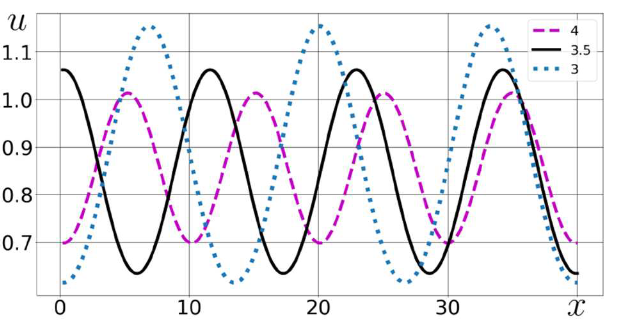
\includegraphics[scale=0.35]{patt_example.png}
        \caption{Пример стационарного негомогенного паттерна}   
        \label{fig:patt_example}   
    }
\end{figure}

В силу того, что гармонические коэффициенты рассчитываются для фиксированного момента времени $t$, их значения меняются вместе с текущим состоянием системы и отслеживание динамики гармонических коэффициентов позволяет эффективно составить представление о характере переходного просцесса. Рис.~\ref{fig:ck_intro} иллюстрирует эту концепцию. 

\begin{figure}[ht]
    \centerfloat{
        \quad\quad\subcaptionbox{Переходный процесс}{%
            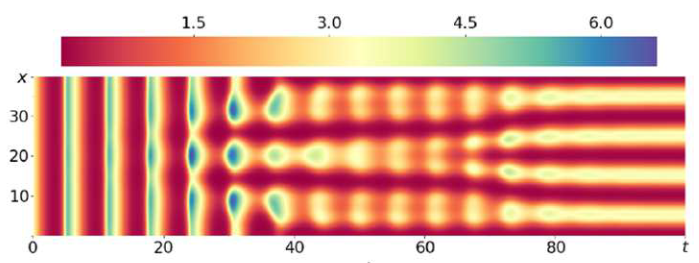
\includegraphics[scale=0.35]{trans_example.png}}
    }
    \\
    \centerfloat{
        \subcaptionbox{Гармонические коэффициенты $C_k$}{%
            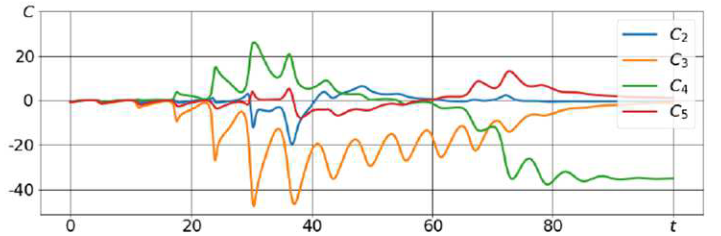
\includegraphics[scale=0.35]{c_k_example.png}}
    }
    \caption{Переходный процесс и его гармонические коэффициенты}\label{fig:ck_intro}
\end{figure}

Можно заметить, что в начальной фазе осцилляций, пока пиковая структура невыражена, коэффициенты близки к нолю, тогда как установившаяся структура с четырьмя пиками сопровождается значительным превышением модуля коэффициента $C_4$ над прочими $C_k$. В силу того, что потенциальное разнообразие количества пиков подобных структур ограничено сверху для конкретной системы и набора её параметров \cite{woolley2017turing}, конечное количество расчитаных $C_k$ позволяет полно описать переходный процесс. Стоит заметить, что доминирующий по модулю $C_k$ даёт хорошее представление о фактическом паттерне сформированном системой даже в присутствии шумов, значительно искажающих вид структуры \cite{bib1}, что делает инструмент гармонических коэффициентов применимым к анализу широкого спектра реальных режимов протекания реакции, для которых присутствие случайного шума является неизбежным в силу воздействия среды. Автоматический расчёт $C_k$ не представляет сложности при наличии снимков состояния переходного процесса, полученных в результате численного эксперимента. Таким образом, при наличии подходящего программного комплекса \cite{progbib2} процесс численного исследования системы и классификации типов паттернов на основе доминирующего $C_k$ может быть выполнен с минимальным участием исследователя.

На основе $C_k$ рассчитанных для результатов численного эксперимента может быть осуществлён анализ всего переходного процесса. Например, смена доминирующего $C_k$ при переходном процессе говорит о том, что состояние системы переместилось к иному аттрактору, например вследствие воздействия шума \cite{bib4}. Также могут быть рассчитаны коэффициенты представленности $W_k$, говорящие о том, насколько был представлен паттерн пиковости $k$ во время конкретного переходного процесса

\begin{equation}
    W_k=\frac{1}{T} \int_0^T C_k^2(t) d t
\end{equation}

Благодаря возможности автоматической детекции образовавшегося паттерна или, наоборот, гомогенной структуры, возможно численно очертить и уточнить фактическую параметрическую зону генерации  паттернов для конкретной системы \cite{bib2}, результат подобного анализа приведён на Рис.~\ref{fig:patt_generation_zone}. При наличии генерации паттернов возможен расчёт относительного количества паттернов каждого вида для данных параметрических условий, что позволяет выделить предпочитаемые системой паттерны и отследить динамику изменения типа предпочитаемого паттерна \cite{bib4}.

\begin{figure}[ht]
    \centerfloat{
        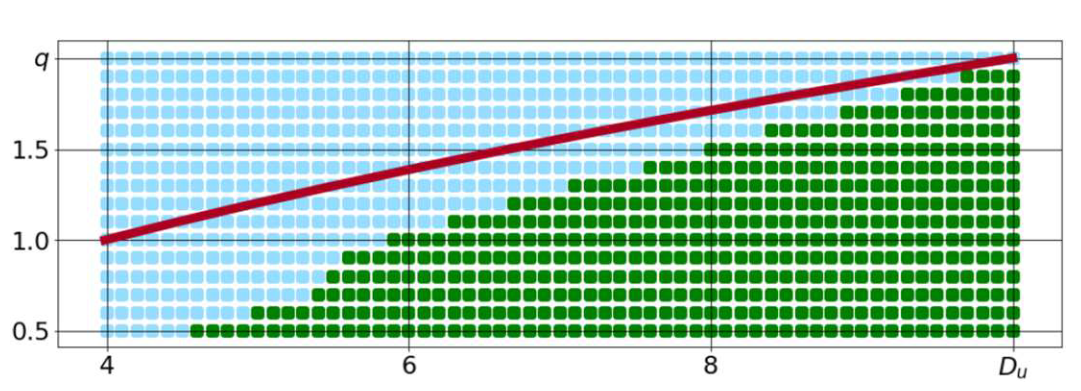
\includegraphics[scale=0.3]{patt_generation_zone.png}
        \caption{Динамические режимы системы. Синие точки означают гомогенные осцилляции, зелёные -- формирование негомогенного устойчивого паттерна.}
        \label{fig:patt_generation_zone}   
    }
\end{figure}

\underline{\textbf{Вторая глава}} посвящена результатам применения вышеописанных механизмов для анализа различных систем, описывающих биохимические процессы, в частности гликолиз. Первый раздел посвящён феноменам, обнаруженным в модели гликолитического осциллятора Хиггинса \cite{higgins1964chemical}

\begin{equation}
    \begin{aligned}
        & \frac{d u}{d t}=1-u v+D_u \frac{\partial^2 u}{\partial x^2} \\
        & \frac{d v}{d t}=p v\left(u-\frac{1+q}{q+v}\right)+D_v \frac{\partial^2 v}{\partial x^2} .
        \end{aligned}
\end{equation}

Для данной системы была аналитически рассчитана бифуркационная диаграмма и описана динамика амплитудных характеристик формируемых паттернов \cite{bib1}. При исследовании параметрической зоны, соответствующей неустойчивой по Тьюрингу конфигурации параметров системы и смежных с ней зон были обнаружены следующие феномены:

\begin{itemize}
    \item \textbf{Мультистабильность в различных конфигурациях}. Показано сосуществование различных комбинаций паттернов аттракторов. Проведён анализ конкретных сосуществующих паттернов для различных параметрических зон.
    \item \textbf{Индуцированные шумом переходы между паттернами}. При воздействии случайного шума на систему возможно изменение режима переходного процесса, выражающееся в смене одного наблюдаемого в течение промежутка времени паттерна-аттрактора на другой, существующий в данной параметрической зоне \cite{bib1}.
    \item \textbf{Предпочтение паттерна в присутствии шума}. Обнаружено, что при воздействии случайного шума в течение переходного процесса система склонна в подавляющем большинстве случаев генерировать паттерн-аттрактор конкретной пиковости. В отсутствии шума подобное предпочтение для той же конфигурации параметров не наблюдается \cite{bib1}.
    \item \textbf{Подавление автоколебаний диффузией}. Показано, что в присутствии диффузии пространственно распределённая модель способна генерировать негомогенные паттерны в параметрической зоне, соответствующей осцилляциям в точечной системе \cite{bib2}.
\end{itemize}

Второй раздел посвящён феноменам, обнаруженным для гликолитического осциллятора Селькова, описываемого системой

\begin{equation}
    \begin{aligned}
        & \frac{d u}{d t}=\vartheta-u v^2+D_u \frac{\partial^2 u}{\partial x^2} \\
        & \frac{d v}{d t}=u v^2-\omega v+D_v \frac{\partial^2 v}{\partial x^2}.
        \end{aligned}
\end{equation}

Для данной системы также была аналитически рассчитана бифуркационная диаграмма и описана динамика амплитудных характеристик формируемых паттернов \cite{bib3}. При подробном исследовании с использованием вышеупомянутых инструментов показано наличие следующих особенностей:

\begin{itemize}
    \item \textbf{Мультистабильность}. Различные конфигурации сосуществующих паттернов-аттракторов были обнаружены для широкого диапазона параметров системы \cite{bib3}, \cite{bib4}.
    \item \textbf{Индуцированная шумом генерация паттернов}. Показано, что в присутствии случайного шума система способна формировать паттерны в параметрической зоне, соответствующей устойчивости по Тьюригу, где в отсутствии шума паттерны не возникают. Обнаружена связь интенсивности шума разнообразием генерируемых системой паттернов \cite{bib3}.
    \item \textbf{Индуцированные шумом переходы между паттернами}. Под воздействием шума система демонстрирует смену негомогенных пространственных конфигураций с течением времени \cite{bib4}.
    \item \textbf{Квантифицировано предпочтение системой некоторых паттернов}. Предложена статистика на основе $C_k$ позволяющая оценить, как уровень случайного шума влияет на время, в течение которого паттерн той или иной пиковости представлен в переходном процессе.
\end{itemize}

Третий раздел посвящён исследованию модели гликолитического осциллятора Селькова-Строгаца

\begin{equation}
    \begin{aligned}
        & \frac{d u}{d t}=-u+a v+u^2 v+D_u \frac{\partial^2 u}{\partial x^2} \\
        & \frac{d v}{d t}=b-a v-u^2 v+D_v \frac{\partial^2 v}{\partial x^2}.
        \end{aligned}
\end{equation}

Для данной системы также была аналитически рассчитана бифуркационная диаграмма и описана динамика амплитудных характеристик формируемых паттернов \cite{bib5}. Применение описанных в первой главе методов позволило описать следующие закономерности:

\begin{itemize}
    \item \textbf{Мультистабильность}. Сосуществование нескольких паттернов-аттракторов при неизменных параметрах системы.
    \item \textbf{Различная энтропия распределения одинаковых конфигураций паттернов}. Для различных параметрических зон может быть характерна одна и та же конфигурация мультистабильности в смысле разнообразия генерируемых системой паттернов-аттракторов. Однако, представляет интерес квантификация предпочтений системы, которая позволила бы отличить ситуацию, когда в подавляющем большинстве случаем система генерирует один тип паттерна, от ситуации, когда генерация любого паттерна из набора потенциально возможных равноверятна. В качестве подобной статистики предложена энтропия \cite{shannon1948mathematical} эмпирического распределения паттернов, сгенерированных системой из случайно возмущённого гомогенного стационарного решения \cite{bib5}.
    \item \textbf{Подавление автоколебаний диффузией в отсутствии шума}. С помощью численных экспериментов было показано, что для данной системы характерно формирование паттернов в присутствии диффузии в т.ч. в зоне автоколебаний точечной системы \cite{bib5}.
\end{itemize}

\underline{\textbf{Третья глава}} посвящена конструированию аналогичного аппарата для автоматической классификации типов паттернов в случае двумерного пространства. Существенная сложность этого случая заключается в том, что наличие двух пространственных координат сильно повышает разнообразие генерируемых паттернов \cite{vanag2004waves}. Некоторые примеры паттернов приведены на Рис.~\ref{fig:2d_patt}. Найти конечный набор базовых элементов, разумная комбинация которых описывает паттерн, становится крайне нетривиальной задачей. 

\begin{figure}[ht]   
    \centerfloat{
        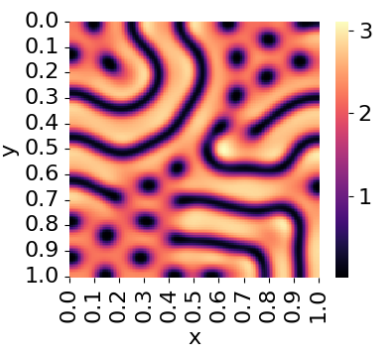
\includegraphics[width=0.33\linewidth]{2d_patt_1.png}
        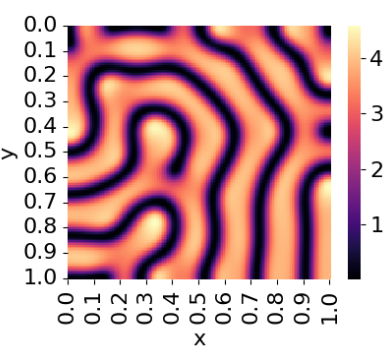
\includegraphics[width=0.33\linewidth]{2d_patt_2.png}
        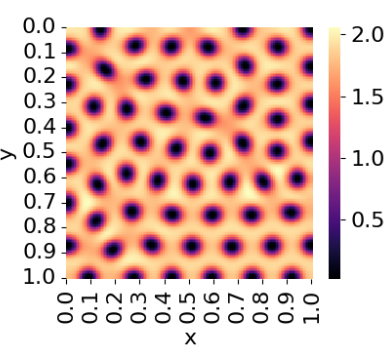
\includegraphics[width=0.33\linewidth]{2d_patt_3.png}  
    \caption{Примеры двумерных паттернов}\label{fig:2d_patt}
    }        
\end{figure}

Вместе с тем исследователи выделяют конечное число типов паттернов, продуцируемых подобными системами \cite{vanag2008book}, \cite{maini2019turing}. В связи с этим представляет интерес инструмент, который, пусть и без претензий на полноту, помог бы автоматически классифицировать известные типы двумерных пространственных паттернов, формируемых динамическими системами в присутствии диффузии. В данной главе предлагается подход к решению такой задачи, позволяющий автоматически классифицировать некоторые типы двумерных структур.

Суть подхода состоит в расчёте подходящих статистик по имеющимся сгенерированномым системой двумерным паттернам. Статистики выбраны так, чтобы с их помощью было возможно описать типы генерируемых системой паттернов без визуального анализа каждого отдельного результата численного эксперимента. Метод состоит в применени следующих шагов:
\begin{itemize}
    \item Бинаризация паттерна по некоторому порогу, для того чтобы выделить структуры. В качестве порога подходит 75-й квантиль значения целевой переменной. Пример паттерна до и после бинаризации приведён на Рис.~\ref{fig:2d_patt_bin}
    \item Детекция элементов, составляющих паттерн с помощью marching squares algorithm \cite{we1987marching}.
    \item Представление каждого элемента как графа. Так как исходный паттерн получен численным решением системы, он представляет собой набор точек. В качестве вершин графа выступают точки, соответствующие рассматриваемому элементу. Рёбра есть между вершинами, соответствующими точкам, соседствующим по вертикали или горизонтали. 
    \item Расчёт диаметра каждого найденного элемента. Под диаметром здесь понимается диаметр графа.
    \item Расчёт статистик на основе набора диаметров элементов, составляющих паттерн. В качестве статистик могут выступать максимальный и средний диаметр. Иллюстрация разделяющей способности этих статистик приведена на Рис.~\ref{fig:2d_stats}, Рис.~\ref{fig:2d_zoo} 
\end{itemize}

\begin{figure}[ht]
    \centerfloat{
        \quad\quad\subcaptionbox{Исходный паттерн}{%
            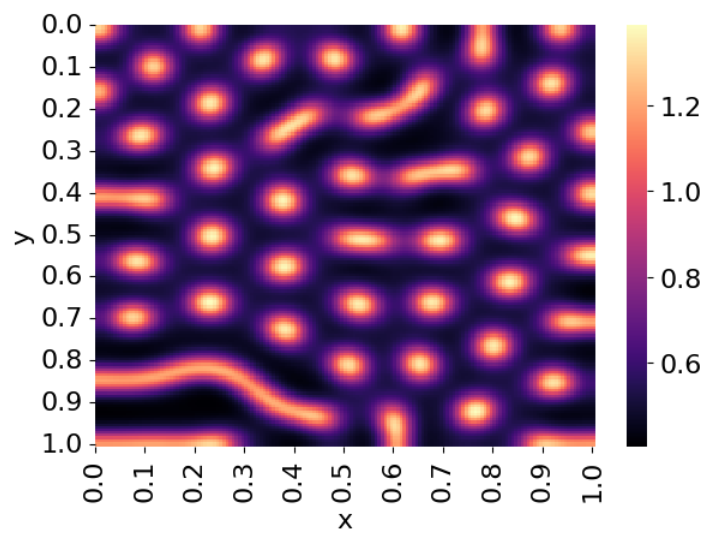
\includegraphics[scale=0.22]{patt_2d.png}}
    }
    \centerfloat{
        \subcaptionbox{Бинаризованый паттерн}{%
            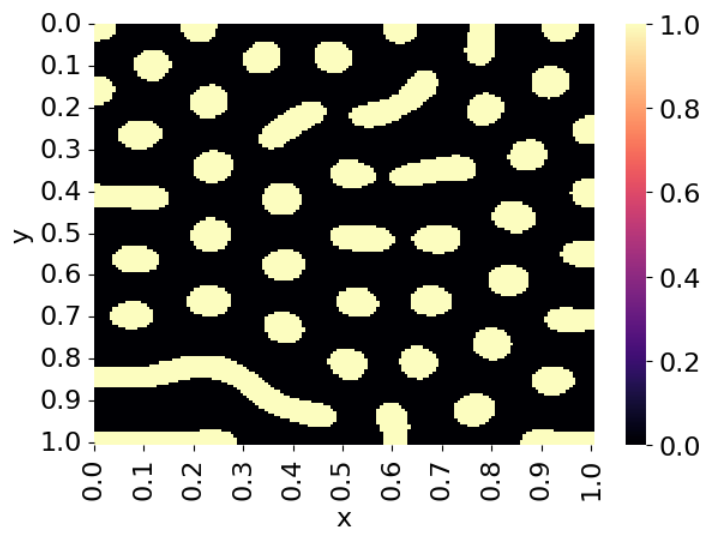
\includegraphics[scale=0.22]{patt_2d_bin.png}}
    }
    \caption{Бинаризация паттерна}\label{fig:2d_patt_bin}
\end{figure}

\begin{figure}[ht]
    \centerfloat{
        \quad\quad\subcaptionbox{Динамика $D_u$}{%
            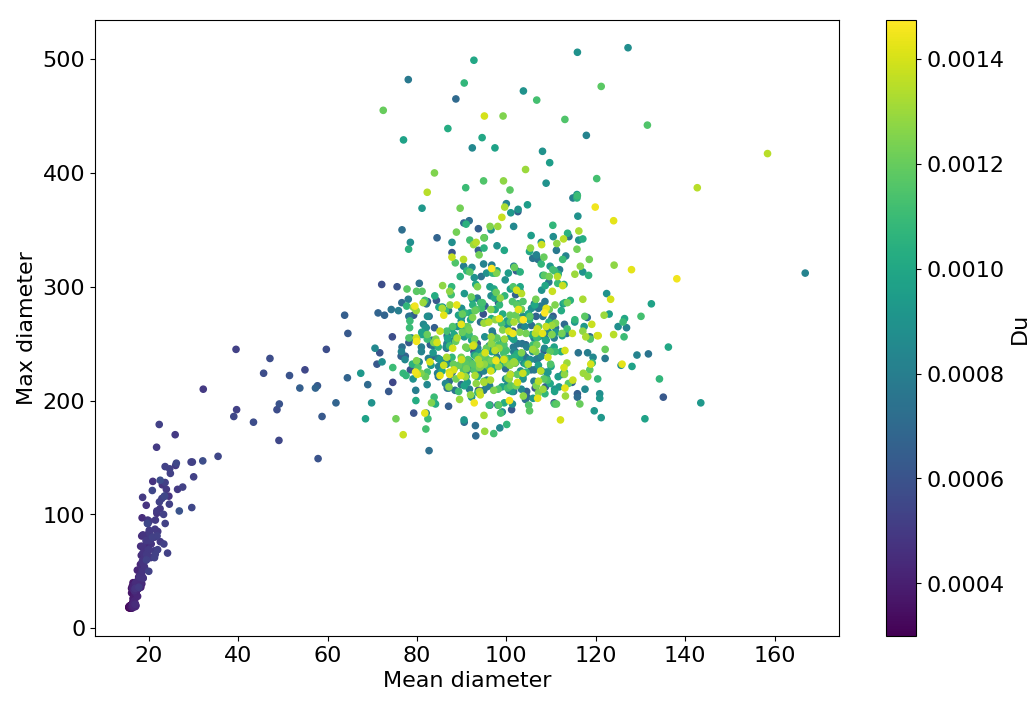
\includegraphics[width=0.55\linewidth]{2d_du.png}}
        \subcaptionbox{Области локализации результатов экспериментов}{%
            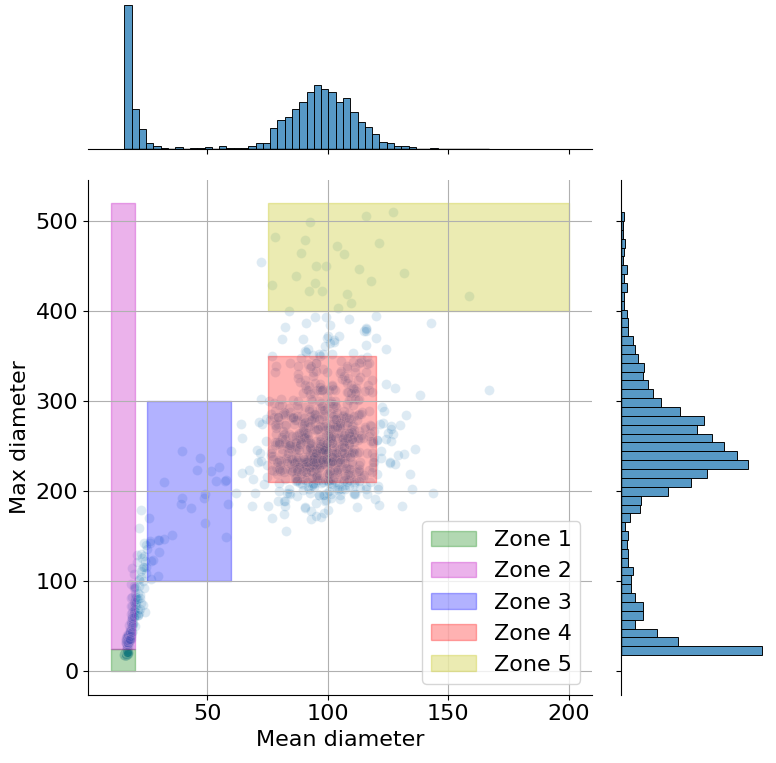
\includegraphics[width=0.44\linewidth]{2d_zones.png}}
    }
    \caption{Результаты численных экспериментов в осях, соответсвующих расчитаным для них статистикам}\label{fig:2d_stats}
\end{figure}

\begin{figure}[ht]
    \centerfloat{
        \subcaptionbox{Паттерн из зоны 1}{%
            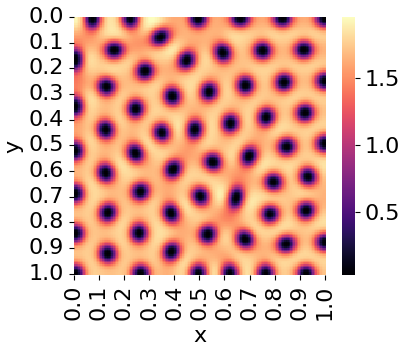
\includegraphics[width=0.3\linewidth]{z1.png}}
    }
    \centerfloat{
        \subcaptionbox{Паттерн из зоны 2}{%
            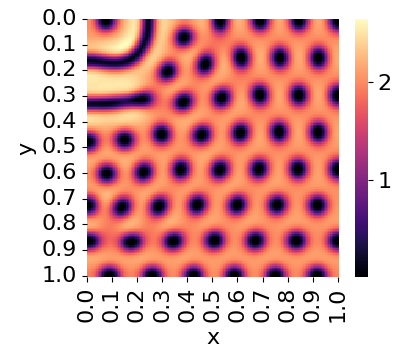
\includegraphics[width=0.3\linewidth]{z2.png}}
    }
    \centerfloat{
        \subcaptionbox{Паттерн из зоны 3}{%
            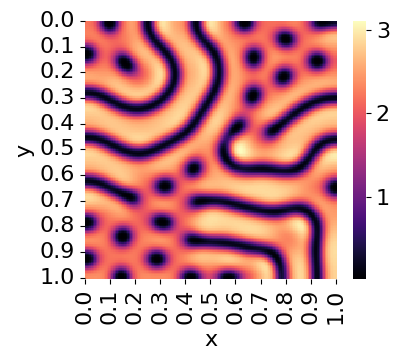
\includegraphics[width=0.3\linewidth]{z3.png}}
    }\\
    \centerfloat{
        \subcaptionbox{Паттерн из зоны 4}{%
            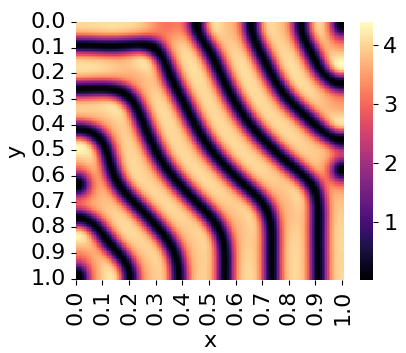
\includegraphics[width=0.3\linewidth]{z4.png}}
    }
    \centerfloat{
        \subcaptionbox{Паттерн из зоны 5}{%
            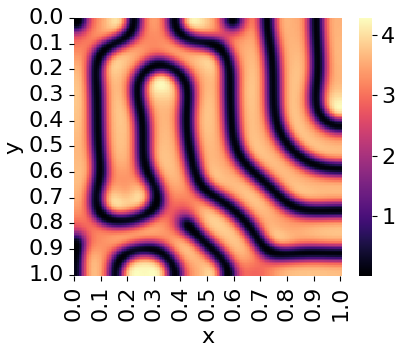
\includegraphics[width=0.3\linewidth]{z5.png}}
    }
    \caption{Примеры паттернов, локализованных в различных зонах в терминах рассчитанных статистик}\label{fig:2d_zoo}
\end{figure}

\FloatBarrier
\pdfbookmark{Заключение}{conclusion}                                  % Закладка pdf
В \underline{\textbf{заключении}} подведены итоги работы, сформулированы выводы и основные результаты. 
%% Согласно ГОСТ Р 7.0.11-2011:
%% 5.3.3 В заключении диссертации излагают итоги выполненного исследования, рекомендации, перспективы дальнейшей разработки темы.
%% 9.2.3 В заключении автореферата диссертации излагают итоги данного исследования, рекомендации и перспективы дальнейшей разработки темы.
\begin{enumerate}
  \item Разработаны методы численного анализа паттернов и переходных процессов в динамических системах с диффузией. 
  \item С помощью разработанных методов исследованы системы гликолитического осциллятора Хиггинса, гликолитического осциллятора Селькова и гликолитического осциллятора Селькова-Строгаца. Рассмотрены как детерминированные переходные процессы, так и поведение систем в присутствии случайного шума.
  \item Для рассмотренных моделей выявлены феномены и особенности генерации паттернов и переходных процессов, результаты опубликованы в рецензируемых изданиях, индексируемых в Scopus.
  \item Разработан программный комплекс, позволяющий проводить и анализировать численные эксперименты с описанными системами. Комплекс позволяет эффективно утилизировать вычислительные ресурсы и анализировать данные, полученные в большом количестве численных экспериментов. Разработанные программы зарегистрированы в реестре программ для ЭВМ.
\end{enumerate}


\pdfbookmark{Литература}{bibliography}                                % Закладка pdf

\ifdefmacro{\microtypesetup}{\microtypesetup{protrusion=false}}{} % не рекомендуется применять пакет микротипографики к автоматически генерируемому списку литературы
\urlstyle{rm}                               % ссылки URL обычным шрифтом
\ifnumequal{\value{bibliosel}}{0}{% Встроенная реализация с загрузкой файла через движок bibtex8
    \renewcommand{\bibname}{\large \bibtitleauthor}
    \nocite{*}
    \insertbiblioauthor           % Подключаем Bib-базы
    %\insertbiblioexternal   % !!! bibtex не умеет работать с несколькими библиографиями !!!
}{% Реализация пакетом biblatex через движок biber
    % Цитирования.
    %  * Порядок перечисления определяет порядок в библиографии (только внутри подраздела, если `\insertbiblioauthorgrouped`).
    %  * Если не соблюдать порядок "как для \printbibliography", нумерация в `\insertbiblioauthor` будет кривой.
    %  * Если цитировать каждый источник отдельной командой --- найти некоторые ошибки будет проще.
    %
    %% authorvak
    \nocite{confbib1}
    \nocite{confbib2}
    \nocite{bib1}
    \nocite{confbib3}
    \nocite{bib2}
    \nocite{confbib4}
    \nocite{bib3}
    \nocite{bib4}
    \nocite{bib5}
    \nocite{progbib1}
    \nocite{progbib2}
   
    \ifnumgreater{\value{usefootcite}}{0}{
        \begin{refcontext}[labelprefix={}]
            \ifnum \value{bibgrouped}>0
                \insertbiblioauthorgrouped    % Вывод всех работ автора, сгруппированных по источникам
            \else
                \insertbiblioauthor      % Вывод всех работ автора
            \fi
        \end{refcontext}
    }{
        \ifnum \totvalue{citeexternal}>0
            \begin{refcontext}[labelprefix=A]
                \ifnum \value{bibgrouped}>0
                    \insertbiblioauthorgrouped    % Вывод всех работ автора, сгруппированных по источникам
                \else
                    \insertbiblioauthor      % Вывод всех работ автора
                \fi
            \end{refcontext}
        \else
            \ifnum \value{bibgrouped}>0
                \insertbiblioauthorgrouped    % Вывод всех работ автора, сгруппированных по источникам
            \else
                \insertbiblioauthor      % Вывод всех работ автора
            \fi
        \fi
        %  \insertbiblioauthorimportant  % Вывод наиболее значимых работ автора (определяется в файле characteristic во второй section)
        \begin{refcontext}[labelprefix={}]
            \insertbiblioexternal            % Вывод списка литературы, на которую ссылались в тексте автореферата
        \end{refcontext}
        % Невидимый библиографический список для подсчёта количества внешних публикаций
        % Используется, чтобы убрать приставку "А" у работ автора, если в автореферате нет
        % цитирований внешних источников.
        \printbibliography[heading=nobibheading, section=0, env=countexternal, keyword=biblioexternal, resetnumbers=true]%
    }
}
\ifdefmacro{\microtypesetup}{\microtypesetup{protrusion=true}}{}
\urlstyle{tt}                               % возвращаем установки шрифта ссылок URL
